\chapter{Team Contribution}
\label{app:contrib}

Table~\ref{tab:contrib} lists the components owned by each member, following the roles assigned in the
project's design document. All members took part in the reviews and are able to explain the complete
system.

\begin{table}[H]
\centering
\caption{Contribution of team members}
\label{tab:contrib}
\small
\begin{tabularx}{\linewidth}{@{}l l X c@{}}
\toprule
\textbf{USN} & \textbf{Name} & \textbf{Components owned} & \textbf{Share} \\ \midrule
\USNa & \NameA\ (Lead) & Project coordination, problem charter, design document, documentation and report & 25\% \\
\USNb & \NameB & Agent and RAG implementation: graph, CaseState, planner, grader, re-planning loop, guardrail, retrieval index, prompts & 25\% \\
\USNc & \NameC & Data collection (GI registry, PIB catalogue, census), simulated records, tools, web interface & 25\% \\
\USNd & \NameD & Golden test set, metrics, baseline, A/B experiment, demonstration tests, error analysis & 25\% \\
\bottomrule
\end{tabularx}
\end{table}

\chapter{Setup and Run Instructions}
\label{app:run}

The source code, the evaluation results and the source of this report are available at
\url{https://github.com/hrterrain/loomtrace-agent}. The system runs on any computer with Python~3.11 or later; no graphics processor or internet
connection is needed in rule mode. The commands below create the environment, start the interface and
reproduce every number in Chapters~7 and~8.

\begin{lstlisting}[language={},numbers=none]
git clone https://github.com/hrterrain/loomtrace-agent.git
cd loomtrace-agent
python3 -m venv .venv && source .venv/bin/activate
pip install -r requirements.txt          # streamlit, langgraph, pydantic, pandas, groq

# optional: enable Llama 3.1 8B on Groq for extraction and explanations
export GROQ_API_KEY=<your key>          # never commit the key

# optional: label images
pip install easyocr

streamlit run app.py                     # web interface on http://localhost:8501
python -m loomtrace.experiments          # Tables 7.1-7.3 and 8.1 -> results/experiments.json
python -m loomtrace.evaluate             # single 45-case evaluation
python run_tests.py                      # 15 demonstration cases -> TEST_RESULTS.md
\end{lstlisting}

Versions used for the reported runs: Python 3.13.7, LangGraph 1.2.20, langchain-core 1.7.7,
Pydantic 2.14.3, Streamlit 1.67.0, pandas 3.1.1, groq 1.7.0, on macOS 15.6 (Apple M2, 8\,GB). The SQLite
database \texttt{loomtrace.db} is created automatically on first run.

\chapter{Sample Traces and Screenshots}

This appendix gives three complete runs: a successful run, a run that required a correction through
re-planning, and an abstention. All were produced by the system on 11 November 2026.

\section{Successful Run with Correction: Kanjivaram Silk Saree}

The node trace of this run is Listing~\ref{lst:replan}, its tool log is Listing~\ref{lst:tools}, and
its checkpoints are Listing~\ref{lst:ckpt}. The first iteration could not resolve the alias
``Kanjivaram'' (grade 0.65); the second resolved it to Kancheepuram Silk, all ten checks passed (grade
1.0), and the verdict \emph{Supported} was issued with seven citations: \texttt{GI15-p3},
\texttt{GI15-p5}, \texttt{GI15-p7}, \texttt{HLCENSUS-2019-20\#Tamil\_Nadu},
\texttt{IPINDIA-GI-REG\#15}, \texttt{SIM-PROV\#B-KAN-0010} and \texttt{SIM-WEAVER\#WV-KAN-001}. The
report shown to the requester is Fig.~\ref{fig:ui}(a).

\section{Contradiction: Banarasi Saree Claimed from Surat}

Listing~\ref{lst:conflict} shows a claim for a Banarasi silk saree said to be made in Surat, Gujarat,
with a valid Banaras weaver and batch. The alias required one re-plan; the verifier then found two
failed checks, and the grader's consistency score of 0 led to \emph{Conflicting evidence}. The report is
Fig.~\ref{fig:ui}(b).

\begin{lstlisting}[language={},caption={Trace of a conflicting claim (case REPORT-TRACE-3)},label={lst:conflict}]
{"node": "Extract",   "msg": "parsed label text: product=Banarasi Silk Saree,
   region=Surat, state=Gujarat, weaver_id=WV-BAN-002, batch_id=B-BAN-0020"}
{"node": "Planner",   "msg": "Initial plan: exact registry match, unfiltered
   document search"}
{"node": "Retriever", "msg": "gi_registry_lookup X . gi_doc_search OK .
   census_lookup OK . weaver_lookup OK . provenance_lookup OK"}
{"node": "Verifier",  "msg": "5 pass . 0 fail . 4 unknown"}
{"node": "Grader",    "msg": "grade=0.69 (completeness 0.56, consistency 1.0)
   -> re-plan"}
{"node": "Planner",   "msg": "Re-plan #1: resolve aliases -> 'Banaras Brocades
   and Sarees', sharper query filtered by product"}
{"node": "Retriever", "msg": "gi_registry_lookup OK . gi_doc_search OK .
   census_lookup OK . weaver_lookup OK . provenance_lookup OK"}
{"node": "Verifier",  "msg": "7 pass . 2 fail . 0 unknown"}
{"node": "Grader",    "msg": "grade=1.0 (completeness 1.0, consistency 0.0)
   -> finish"}
{"node": "Guardrail", "msg": "Conflicting evidence"}
rationale: "Conflict found: Region 'Surat' is NOT in GI area (Varanasi,
  Mirzapur, Chandauli, Bhadohi, Jaunpur, Azamgarh); State 'Gujarat' vs
  registered 'Uttar Pradesh'."
\end{lstlisting}

\section{Abstention: Banaras Saree without Producer Details}

The trace of this run is Listing~\ref{lst:hitl}. Figure~\ref{fig:insuff} shows the report presented to
the requester, which states that the case has been sent to an expert reviewer and lists the four
producer checks that could not be made. The reviewer's dashboard and the requester's tracking view for
such a case are Figs.~\ref{fig:admin} and~\ref{fig:track}.

\begin{figure}[H]
\centering
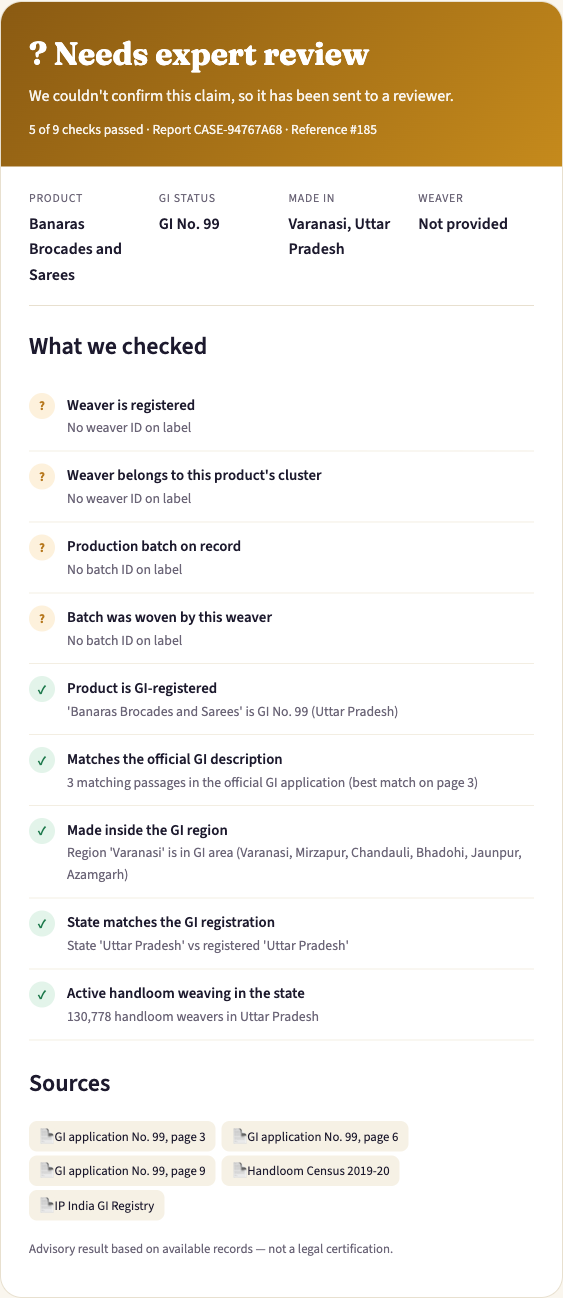
\includegraphics[width=0.5\linewidth]{figures/ui_insufficient.png}
\caption{Report for a claim without weaver or batch details, escalated to human review}
\label{fig:insuff}
\end{figure}

\chapter{Prompts}
\label{app:prompts}

LoomTrace uses a language model only in the optional model mode, for two tasks. Both prompts are sent
as the system message to \texttt{llama-3.1-8b-instant} on Groq with temperature 0 and
\texttt{response\_format=\{"type": "json\_object"\}}. As stated in Section~6.5, these prompts were not
used in the reported evaluation. No model is used as a judge, so there is no judge rubric.

\begin{lstlisting}[language={},caption={System prompt for field extraction; the user message is the label text}]
Extract handloom label fields. Return JSON with keys: product, region (district),
state, weaver_id, batch_id, material, gi_claim (bool). Use null if absent.
Copy IDs exactly.
\end{lstlisting}

\begin{lstlisting}[language={},caption={System prompt for the verdict explanation; the user message is a JSON object with the verdict, the status of each check and up to twelve source IDs with notes}]
You explain a GI verification verdict in 2-3 sentences. Only use the given checks
and cite sources in [brackets]. Return JSON {"rationale": str}.
\end{lstlisting}

The extraction prompt asks for a fixed key set so that the output can be validated by the
\texttt{LabelFields} model, requires \texttt{null} for absent fields so that missing information is not
invented, and requires identifiers to be copied exactly because they are used as database keys. The
explanation prompt limits the model to the checks already computed, so that the explanation cannot
introduce facts that were not verified. If either call fails or returns invalid JSON, the deterministic
parser or the template explanation is used instead.
